% !TEX program = pdflatex
\documentclass[aspectratio=169,11pt]{beamer}

% -----------------------
% Theme
% -----------------------
\usetheme{Madrid}
\usecolortheme{default}
\setbeamertemplate{navigation symbols}{}

% -----------------------
% Packages
% -----------------------
\usepackage[english]{babel}
\usepackage{graphicx}
\usepackage{transparent}
\usepackage{tikz}
\usepackage{xcolor}
\usepackage{hyperref}

\graphicspath{{figures/}}

% -----------------------
% Colors (red only; no orange)
% -----------------------

% Avoid ugly hyphenation in title
\hyphenpenalty=10000
\exhyphenpenalty=10000

% -----------------------
% Metadata (your fields)
% -----------------------
\author{G.V. Vetsler}
\title[Comparing collaborative filtering models]{Comparing classical and neural collaborative filtering models\\on implicit feedback data}
\newcommand\subtitletext{Comparing collaborative filtering models}


\newcommand\supervisor{Dr. Marijn Jansen}
\newcommand\secondexaminer{Dr. Tamas Vinko}
\date{\today}

% -----------------------
% Tunables (easy to adjust)
% -----------------------
\newcommand{\HeaderShift}{8.2cm}      % move header block right
\newcommand{\TitleFont}{10}
\newcommand{\TitleLeading}{8}      % title line spacing (pt)

\begin{document}

% =======================
% Title page
% =======================
\begin{frame}[plain]

% Background image (expects images/bg.png)
\begin{tikzpicture}[remember picture,overlay]
  \node[anchor=center,opacity=0.35] at (current page.center)
    {
\includegraphics[height=0.85\paperheight]{titlepage_background.png}};
\end{tikzpicture}

% White mask panel (top-left) to prevent background/text interference
\begin{tikzpicture}[remember picture,overlay]
  \fill[white,opacity=0.92]
    ([xshift=0.0cm,yshift=0.0cm]current page.north west)
    rectangle
    ([xshift=0.64\paperwidth,yshift=-0.36\paperheight]current page.north west);
\end{tikzpicture}

% UCR logo (expects images/UCRlogo.png)
\begin{tikzpicture}[remember picture,overlay]
  \node[anchor=north west,xshift=0.55cm,yshift=-0.55cm] at (current page.north west)
    {\transparent{0.35}
\includegraphics[height=0.85cm]{ucr_logo.png}};
\end{tikzpicture}

\begin{flushleft}

% Header block (moved right)
\begin{minipage}{\textwidth}
  \hspace*{\HeaderShift}%
  \begin{minipage}{0.85\textwidth}
    {\Large{University College Roosevelt}}\\[-0.05cm]
    {\scriptsize Lange Noordstraat 1, Middelburg, The Netherlands}\\[-0.05cm]
    {\scriptsize Bachelor of Liberal Arts \& Sciences}
  \end{minipage}
\end{minipage}
\vspace{0.35cm}

% Senior Project + rule (NOT moved right)
{\Large {Senior Project}}\\[-0.10cm]
{\color{UCRred}\rule{\textwidth}{0.6pt}}
\vspace{0.16cm}


% Title + subtitle
\begin{minipage}{0.94\textwidth}
  {\fontsize{\TitleFont}{\TitleLeading}\selectfont\bfseries
   {\inserttitle}\par}
  \vspace{0.05cm}
  {\normalsize \subtitletext\par} % subtitle in black
\end{minipage}

\vspace{0.14cm}
{\rule{\textwidth}{0.6pt}}
\vspace{0.3cm}
% Info block (compact)
% Info block (tighter spacing)
\begin{minipage}{0.70\textwidth}
\scriptsize

\textbf{\textcolor{UCRred}{Author:}}\\[-0.05cm]
\insertauthor\\[0.10cm]

\textbf{\textcolor{UCRred}{Supervisor:}}\\[-0.05cm]
\supervisor\\[0.10cm]

\textbf{\textcolor{UCRred}{Second examiner:}}\\[-0.05cm]
\secondexaminer\\[0.12cm]

\insertdate
\end{minipage}

\end{flushleft}
\end{frame}



% =======================
% Talk map
% =======================
\begin{frame}{Table of contents}
\begin{enumerate}
  \item Motivation and problem setting
  \item Data and evaluation protocol
  \item Models (classical and neural)
  \item Results (MovieLens vs Yelp)
  \item Conclusions, limitations
\end{enumerate}
\end{frame}

% =======================
% Problem
% =======================
\begin{frame}{The problem: recommending from implicit feedback}
Real systems: Netflix, Spotify, TikTok, Yelp, e-commerce.\\
They observe mostly implicit signals: clicks, views, purchases.

\medgap
Key challenge: ``No interaction'' does \alert{not} mean dislike.\\
So we treat recommendation as a ranking problem: what should be top for each user?

\begin{figure}[H]
    \centering
    
\includegraphics[width=0.3\linewidth]{netflix_homepage.png}
    \caption{Netflix recommendation page. Source: Figma Community — Netflix Home Page (Desktop \& TV).}
    \label{fig:netflix}
\end{figure}
\end{frame}
% =======================
% Collaborative Filtering in one slide
% =======================
\begin{frame}{Collaborative Filtering in one slide}
Core idea: recommend items using \emph{other users’ behavior}, not item content.

\begin{figure}[H]
    \centering
    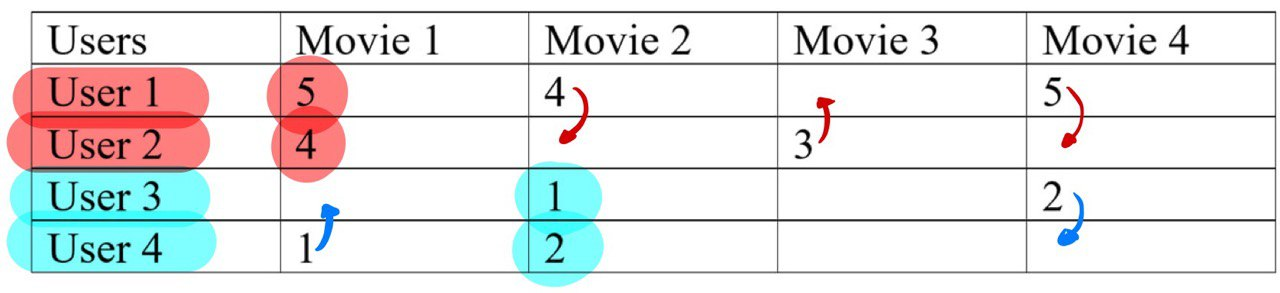
\includegraphics[width=0.5\linewidth]{cf_illustration.png}
    \caption{Example of the Collaborative filtering idea}
    \label{fig:placeholder}
\end{figure}
If User 1 and User 2 both liked Movies 1 and 2, and User 1 also liked Movie 4,\\
then Movie 4 becomes a good candidate recommendation for User 2.
\end{frame}


% =======================
% Data overview
% =======================
\begin{frame}{Datasets}
\begin{block}
  
\begin{itemize}
  \item MovieLens-1M (movies): denser interactions, Movies vs Users
  \item Yelp (businesses): much sparser, local/business structure, geographical semantics
\end{itemize}

\end{block}
\medgap

\begin{columns}[T,onlytextwidth]
\column{0.49\textwidth}
\centering
\small MovieLens-1M 
\medskip

\scriptsize
\begin{tabular}{lr}
\toprule
Users ($M$) & 6{,}040 \\
Items ($N$) & 3{,}706 \\
Interactions & 1{,}000{,}209 \\
Density & 4.4684\% \\
Sparsity & 95.5316\% \\
Avg. / user & 165.60 \\
Avg. / item & 269.89 \\
\bottomrule
\end{tabular}

\column{0.49\textwidth}
\centering
\small Yelp 
\medskip

\scriptsize
\begin{tabular}{lr}
\toprule
Users ($M$) & 24{,}930 \\
Items ($N$) & 25{,}799 \\
Interactions & 690{,}381 \\
Density & 0.1073\% \\
Sparsity & 99.8927\% \\
Avg. / user & 27.69 \\
Avg. / item & 26.76 \\
\bottomrule
\end{tabular}
\end{columns}



\end{frame}
\begin{frame}{Models compared}
Classic baselines:
\begin{itemize}
  \item ItemKNN: recommend items similar to what you liked
\end{itemize}
MF models:
\begin{itemize}
   \item MF-BPR: matrix factorization trained for ranking (BPR)
     \item GMF: shallow neural MF variant
\end{itemize}
\medgap
Neural CF family:
\begin{itemize}

  \item MLP: non-linear interaction function
  \item NeuMF: GMF + MLP hybrid (with and without pretraining)
\end{itemize}

\medgap
ConvNCF:
\begin{itemize}
  \item outer product $\rightarrow$ interaction map $\rightarrow$ CNN
\end{itemize}
\end{frame}


% =======================
% Matrix Factorization (MF)
% =======================
\begin{frame}{Matrix Factorization (MF): the classic baseline}
Idea: represent each user and item with a low-dimensional vector (embedding).

\medgap
\begin{itemize}
  \item User $u$ has embedding $\mathbf{p}_u \in \mathbb{R}^k$, item $i$ has embedding $\mathbf{q}_i \in \mathbb{R}^k$.
  \item Predicted preference score:
  \[
    \hat{y}_{ui} = \mathbf{p}_u^\top \mathbf{q}_i
  \]
  \item Interpretation: if vectors align, the score is high (good match).
  \item Limitation: interaction is linear (dot product) $\rightarrow$ cannot directly model complex non-linear patterns.
\end{itemize}

\medgap
\begin{block}{Link to GMF}
GMF is a neural generalization of MF: it replaces the fixed dot product with a learnable weighted element-wise interaction, while staying almost as simple.
\end{block}
\medgap
\begin{block}{MF-BPR}
Same MF scoring function, but trained to rank observed items above unobserved ones using BPR loss.
\end{block}
\end{frame}




% =======================
% NeuMF visual (placeholder)
% =======================
\begin{frame}{NeuMF in one picture (hybrid model)}
\begin{columns}[T,onlytextwidth]
  \column{0.55\textwidth}
  \textbf{Idea:} keep MF-like interaction \emph{and} add non-linear capacity.
  \begin{itemize}
    \item GMF branch: element-wise product
    \item MLP branch: concatenation + dense layers
    \item Fuse at output
  \end{itemize}

  \medgap
  \textbf{Pretraining variant:} train GMF and MLP first, then use their weights to initialize NeuMF.

  \column{0.45\textwidth}
  \centering
  % Use your existing image name if available
  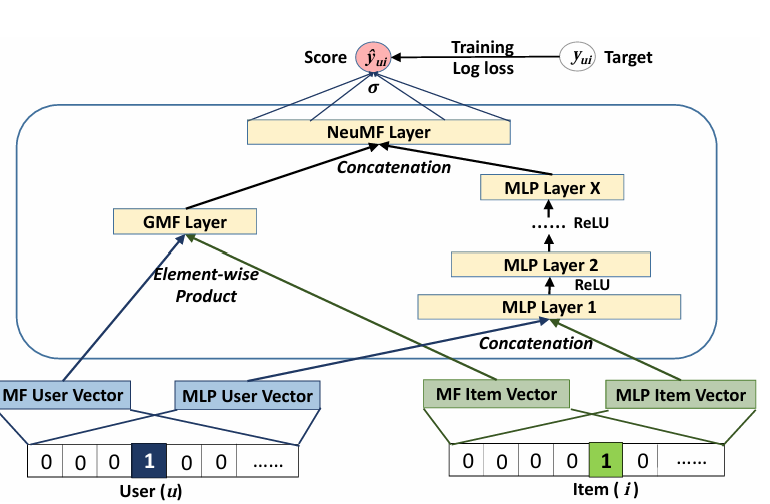
\includegraphics[width=\linewidth]{neumf_architecture.png}\\
   \caption{Schematic illustration of the NeuMF architecture combining GMF and MLP.(Figure adapted from ~\cite{he2017neural}).}
\end{columns}
\end{frame}

% =======================
% CNN explanation (with interaction map figure)
% =======================
\begin{frame}{Why CNN shows up in recommendation (ConvNCF intuition)}
\begin{columns}[T,onlytextwidth]
\column{0.58\textwidth}
\textbf{CNN = processes images / 2D patterns.}

\medgap
ConvNCF creates a 2D ``image'' from embeddings:
\[
\mathbf{E}_{ui} = \mathbf{p}_u \mathbf{q}_i^\top \in \mathbb{R}^{k \times k}
\]
\textbf{Claim:} this interaction map contains local patterns a CNN can detect.

\medgap
\begin{block}{Key skepticism}
Unlike pixels in images, embedding dimensions have no natural spatial order.
\end{block}

\column{0.42\textwidth}
\centering
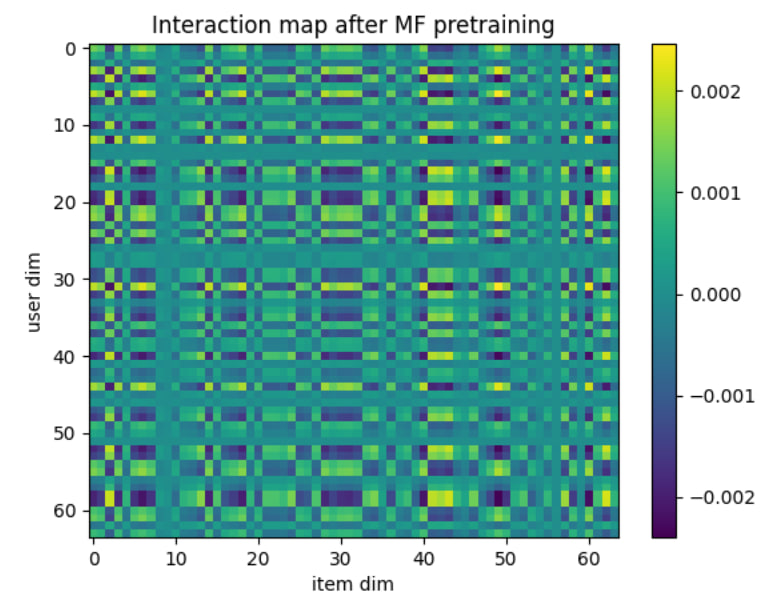
\includegraphics[width=\linewidth]{mf_heatmap_movielens.png}
\scriptsize
\medskip

Interaction map (outer product of embeddings) after MF pretraining (MovieLens)
\end{columns}
\end{frame}


% =======================
% ConvNCF architecture visual (placeholder)
% =======================
\begin{frame}{ConvNCF architecture (outer product $\rightarrow$ CNN)}
\begin{columns}[T,onlytextwidth]
  \column{0.55\textwidth}
  \textbf{Pipeline:}
  \begin{enumerate}
    \item user/item embeddings
    \item outer product $\rightarrow$ $k\times k$ interaction map
    \item several Conv2D layers
    \item flatten + output
  \end{enumerate}

  \smallgap
  \textbf{In this thesis:} a \alert{shallow} ConvNCF variant: \{32,32,64\} filters, (compute constraints).

  \column{0.45\textwidth}
  \centering
  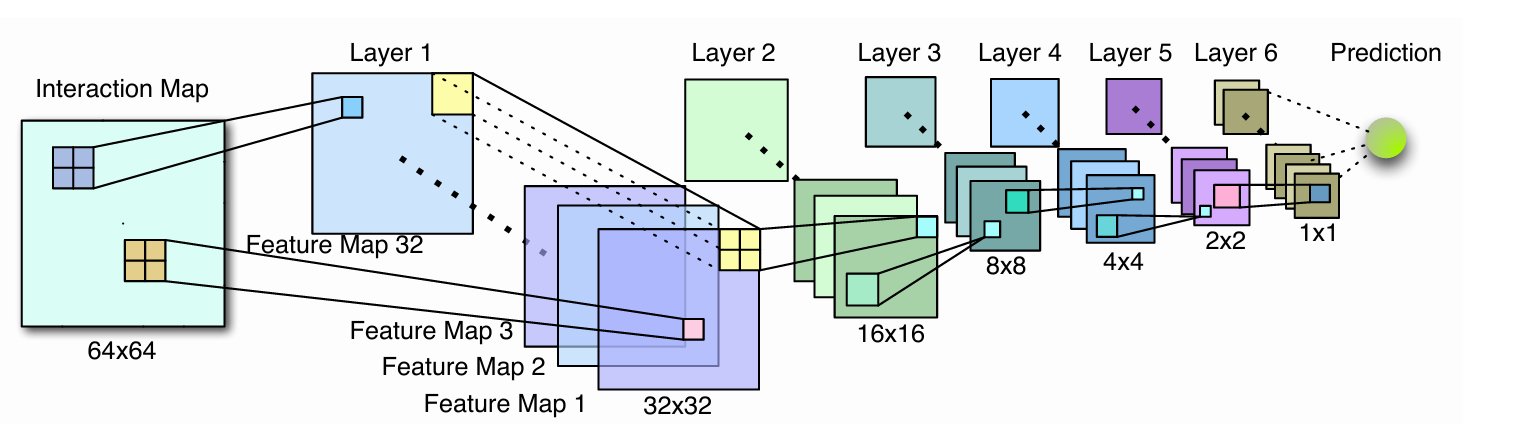
\includegraphics[width=\linewidth]{convncf_architecture.png}\\
  \caption{An example of the architecture of our ConvNCF model that has 6 convolution layers with embedding size 64 (Figure adapted from \cite{he2018convncf}).}
\end{columns}
\end{frame}




% =======================
% Training setup (high level)
% =======================
\begin{frame}{Training setup (high level)}
Negative sampling: for each positive interaction, sample unobserved items as negatives.

\medgap
Two training objectives:
\begin{itemize}
  \item Pointwise (GMF / MLP / NeuMF): classify observed vs sampled unobserved (negative)
  \item Pairwise BPR (MF-BPR / ConvNCF): rank positive above negative
\end{itemize}
Hyperparameter search: For NeuMF and ConvNCF models a limited hyperparameter search was conducted\\
Best weights search: Using validation dataset, pick the best weights.
\end{frame}

% =======================
% Evaluation protocol
% =======================
\begin{frame}{Evaluation protocol}
Leave-one-out:
\begin{itemize}
  \item For each user, hold out the most recent interaction as test
  \item Add 99 randomly sampled negatives for evaluation
  
  \item Validate using the same protocol on the next most recent interaction
  \item Train on the remaining interactions
  
\end{itemize}

\medgap
Ranking metrics at $K=10$:\\
Predict 10 items, per user:
\begin{itemize}
  \item HR@10: how many true items are in those Top-10?
  \item NDCG@10: rewards placing the true item higher in the Top-10
\end{itemize}
\end{frame}

% =======================
% Research questions
% =======================
\begin{frame}{Research questions}
\begin{enumerate}
  \item Are MLP-based models a good fit for CF?
  \item Is ConvNCF a good fit and the outer product actually has spatial
features that can be captured by CNNs?
  \item To what extent deep learning is helpful in the CF models?
\end{enumerate}
\end{frame}
% =======================
% Training / validation curves (split into two slides)
% =======================

% ---------- Slide 1: NeuMF on MovieLens (training + validation) ----------
\begin{frame}{Training dynamics: NeuMF on MovieLens}
\scriptsize

\begin{columns}[T,onlytextwidth]
\column{0.50\textwidth}
\centering
NeuMF training (loss + accuracy)
\medskip

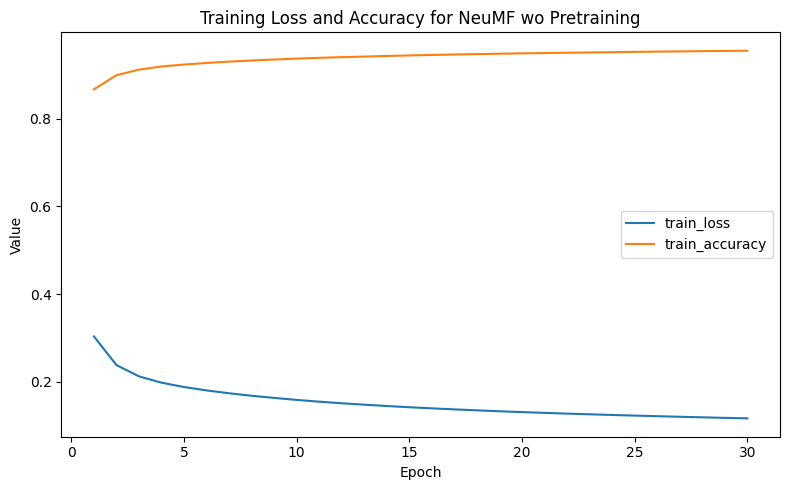
\includegraphics[width=\linewidth]{neumf_movielens_train.png}
\caption{NeuMF on MovieLens: training loss and training accuracy over epochs.}

\column{0.50\textwidth}
\centering
NeuMF validation (HR@10 + NDCG@10)
\medskip

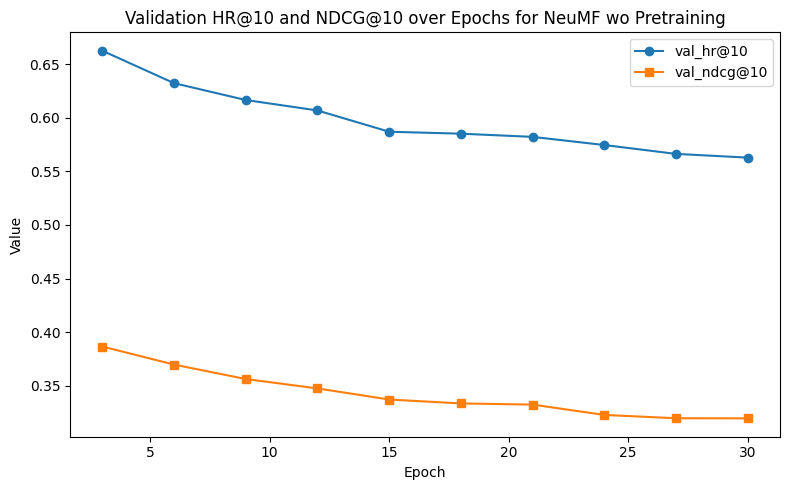
\includegraphics[width=\linewidth]{neumf_movielens_val.png}
\caption{NeuMF on MovieLens: validation HR@10 and NDCG@10 (evaluated every 3 epochs).}
\end{columns}

\end{frame}


% ---------- Slide 2: ConvNCF on Yelp (training + validation) ----------
\begin{frame}{Training dynamics: ConvNCF on Yelp}
\scriptsize

\begin{columns}[T,onlytextwidth]
\column{0.50\textwidth}
\centering
ConvNCF training (loss + accuracy)
\medskip

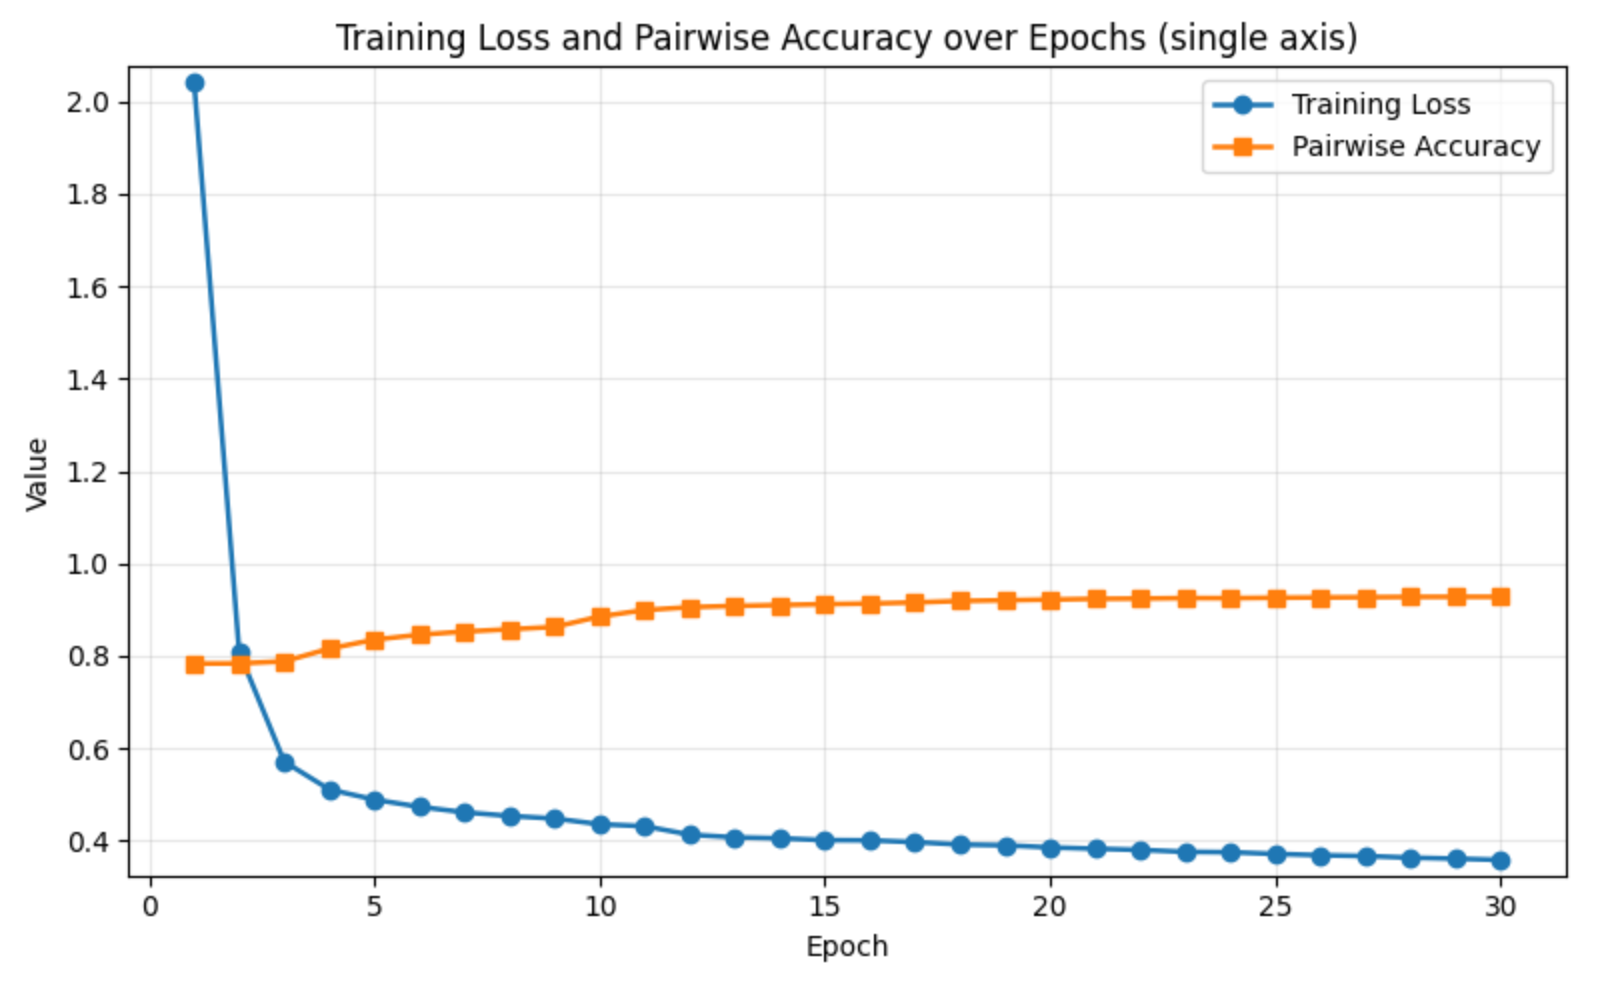
\includegraphics[width=\linewidth]{convncf_yelp_train.png}
\caption{ConvNCF on Yelp: training loss and training accuracy over epochs.}

\column{0.50\textwidth}
\centering
ConvNCF validation (HR@10 + NDCG@10)
\medskip

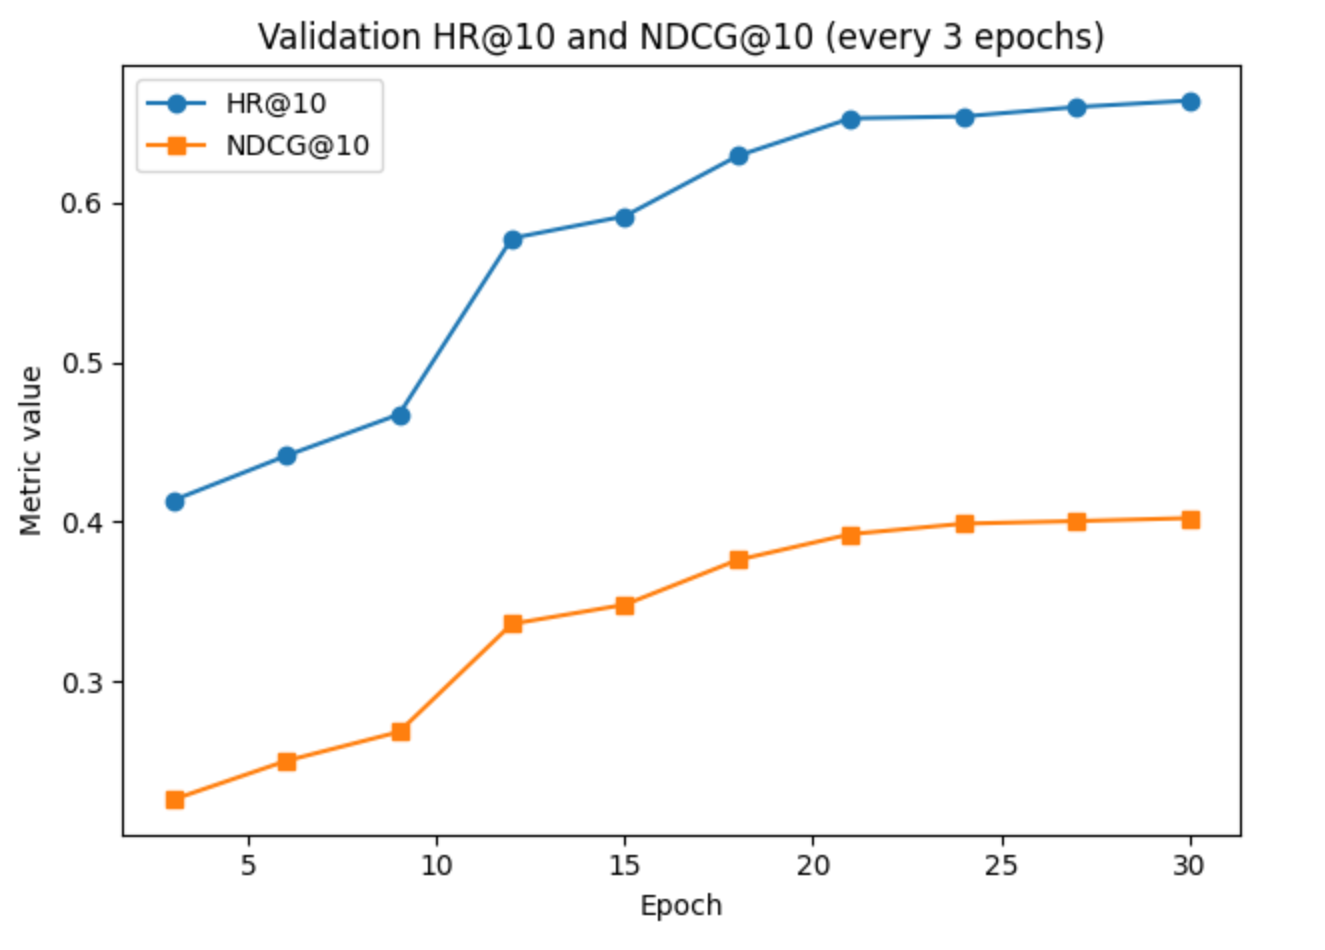
\includegraphics[width=\linewidth]{convncf_yelp_val.png}
\caption{ConvNCF on Yelp: validation HR@10 and NDCG@10 (evaluated every 3 epochs).}
\end{columns}

\end{frame}


% =======================
% Results: MovieLens
% =======================
\begin{frame}{Results on MovieLens-1M (top-10 accuracy)}
\textbf{Metric focus:} HR@10 and NDCG@10 (higher is better)

\medgap
\centering
\begin{tabular}{lcc}
\toprule
Model & HR@10 & NDCG@10 \\
\midrule
\textbf{GMF}        & \textbf{0.6629} & \textbf{0.3853} \\
NeuMF-pre  & 0.6480 & 0.3814 \\
NeuMF      & 0.6457 & 0.3752 \\
MLP        & 0.6358 & 0.3675 \\
ItemKNN    & 0.5204 & 0.3022 \\
MF-BPR     & 0.5379 & 0.2989 \\
ConvNCF    & 0.3220 & 0.1606 \\
\bottomrule
\end{tabular}

\medgap
\begin{block}{Interpretation}
On MovieLens, the \alert{simpler} embedding-based model (GMF) is best.\\
ConvNCF fails badly: high complexity, low generalization.
\end{block}
\end{frame}

% =======================
% Results: Yelp
% =======================
\begin{frame}{Results on Yelp (top-10 accuracy)}
\textbf{Metric focus:} HR@10 and NDCG@10

\medgap
\centering
\begin{tabular}{lcc}
\toprule
Model & HR@10 & NDCG@10 \\
\midrule
\textbf{ItemKNN}    & \textbf{0.7301} & \textbf{0.4747} \\
NeuMF-pre  & 0.6917 & 0.4297 \\
MLP        & 0.6787 & 0.4224 \\
GMF        & 0.6775 & 0.4284 \\
NeuMF      & 0.6744 & 0.4264 \\
ConvNCF    & 0.6242 & 0.3702 \\
MF-BPR     & 0.4329 & 0.2666 \\
\bottomrule
\end{tabular}

\medgap
\begin{block}{Interpretation}
On Yelp, a \alert{classic} baseline (ItemKNN) wins.\\
Neural MF-style models are competitive but do not dominate.
\end{block}
\end{frame}


\begin{frame}{RQ1: Are MLP-based models a good fit for CF?}
\begin{itemize}
  \item MLP-based models (MLP, NeuMF) are competitive, but not consistently better than simpler MF-style models.
  \item On MovieLens, GMF achieves the best ranking quality (highest NDCG@10); NeuMF variants are close but not dominant.
  \item Validation curves often peak early and then decline $\rightarrow$ higher capacity can translate into overfitting.
  \item Pretraining helps NeuMF, but the improvement is modest.
  \item This matches prior findings that strong MF-style baselines remain highly competitive and that gains from neural CF can be small under fair evaluation \cite{rendle2020neural,anelli2021reenvisioning}.
\end{itemize}

\medgap
\begin{block}{Takeaway}
More non-linearity does not automatically translate into better top-$K$ recommendations.
\end{block}
\end{frame}


\begin{frame}{RQ2: Is ConvNCF a good fit, and does the outer product have CNN-friendly patterns?}
\begin{itemize}
  \item MovieLens: ConvNCF generalizes very poorly (low and unstable validation metrics), despite fitting training data well.
  \item Yelp: ConvNCF works better than on MovieLens, but still lags behind strong baselines and MF-style neural models.
  \item Core concern: CNNs assume spatial locality, but embedding dimensions have no natural order.
  \item Even where ConvNCF improves (Yelp), a simple ItemKNN baseline remains stronger.
  \item This aligns with replication-based critiques arguing that CNN locality assumptions do not naturally apply to embedding interaction maps \cite{anelli2021reenvisioning}.
\end{itemize}

\medgap
\begin{block}{Takeaway}
The CNN inductive bias does not reliably match the structure of outer-product interaction maps.
\end{block}
\end{frame}


\begin{frame}{RQ3: How much does deep learning help vs well-tuned classical baselines?}
\begin{itemize}
  \item On MovieLens, embedding-based models (especially GMF) clearly beat classical baselines (KNN, MF-BPR).
  \item Extra architectural complexity (MLP depth, CNNs) yields small or negative gains under limited tuning.
  \item On Yelp, strong neighbourhood structure makes ItemKNN the best accuracy model.
  \item NeuMF-pre is robust and competitive, but not a universal winner across both dataset types.
  \item Overall, this supports the broader message that careful baselines and fair evaluation are essential when claiming neural CF improvements \cite{rendle2020neural,anelli2021reenvisioning}.
\end{itemize}

\medgap
\begin{block}{Takeaway}
Deep learning helps mainly via good embeddings and training, not automatically via complexity.
\end{block}
\end{frame}



% =======================
% Limitations
% =======================
\begin{frame}{Limitations}
\begin{itemize}
  \item \textbf{Restricted hyperparameter search:} deep models are sensitive (LR, L2, batch size, sampler).
  \item \textbf{Training horizon:} some models improve with longer training (ConvNCF in original work trains very long).
  \item \textbf{ConvNCF variant:} shallow CNN used (stability/compute constraints).
  \item \textbf{Negative sampling:} simple uniform sampling; smarter/harder negatives may change outcomes.
  
\end{itemize}
\end{frame}



% =======================
% Final slide
% =======================
\begin{frame}{Conclusion}
\begin{block}{}
Under controlled conditions and limited tuning budget:
\begin{itemize}
  \item \textbf{NeuMF} is competitive, but does not consistently beat simpler models.
  \item \textbf{GMF} (shallow) is best on MovieLens.
  \item \textbf{ItemKNN} is best on Yelp.
  \item \textbf{ConvNCF} does not justify its complexity in this setup.
\end{itemize}
\end{block}


\end{frame}

\begin{frame}{Acknowledgments}
\begin{itemize}
  \item I would like to thank Dr. Marijn Jansen for supervision, guidance, and feedback throughout this project.
  \item Thank you for your attention.
\end{itemize}
\end{frame}

% =======================
% References (short, talk-friendly)
% =======================
\begin{frame}[allowframebreaks]{References}
\bibliographystyle{plain}
\bibliography{references}
\end{frame}

\end{document}
